\section{Question 2}
\paragraph{}
Consider the following potential

$$
	V(\phi) = \frac{\lambda}{4}(\phi^2 - v^2)^2
$$

where $\lambda > 0$ and $v > 0$. Plot this potential, and show that the minima of this potential is at $\phi_{min}=\pm v$.

\begin{figure}[H]
    \centering
    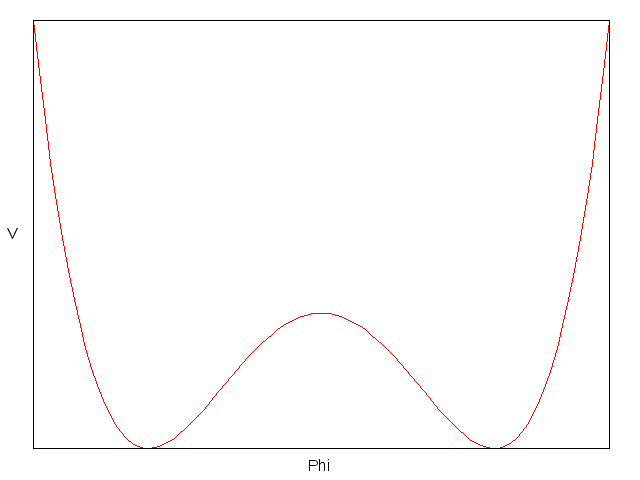
\includegraphics[width=0.5\textwidth]{q2-potential.png}
    \caption{Potential}
    \label{fig:q2-potential}
\end{figure}
%
\paragraph{}
Turning points of a function may be found when the first derivative of the function is equal to zero.

$$
	\frac{\partial V(\phi) } {\partial \phi}
	= \frac{\lambda}{4} 2 (\phi^2 - v^{2}) 2 \phi
	= \lambda (\phi^2 - v^{2}) \phi
$$

It can be seen that when this derivative is equal to zero that there are three possible solutions at $\phi=0$ and $\phi=\pm v^{2}$.  In order to identify which points are minima it is necessary to evaluate the second derivative of the potential at each of these points.

$$
	\frac{\partial ^2 V(\phi) } {\partial \phi ^2}
	= \lambda (\phi^{2} - v^{2}) + 2 \lambda \phi
$$

Evaluating the second derivateive at these points shows that the minima of this function are at $\phi=\pm v^{2}$ and that there is a maximum at $\phi=0$.


\paragraph{}
Considering the static solutions, where $\dot{\phi} = \ddot{\phi} = 0$. The Klein-Gordon Equation in this limit is then

$$
	\frac{\partial ^2 \phi } {\partial x^2} - \lambda (\phi ^{2} - v^{2})\phi = 0
$$

Showing that the \textit{vacuum} solution, where $\phi(x,t) = \pm v$, satisfies the static Klein-Gordon Equation is as simple as substituting $\phi$ into the equation.  As the value for $\phi$ is a constant it is clear that $\partial_x \phi$ is zero along with all higher order derivatives.  This simplifies the solving of the equation.

$$
	(0) - \lambda \bigg((\pm v) ^{2} - v^{2} \bigg)(\pm v)
	= 0
$$

\paragraph{}
Changing $\phi$ to the following where m = $\sqrt{\lambda}v$ and $x_0$ are constants is known as the kink solution.

$$
	\phi^{+} (x) = v tanh \bigg[ \frac{m}{\sqrt{2}}(x - x_0) \bigg]
$$

\paragraph{}
Having shown that the kink solultion does indeed satisfy the static Klein-Gordon equation one wonders what other equations will do so.  It is possible to check a for a few more solutions simply by changing the parity of the solution.  If this is possible it should be possible to show that the static Klein-Gordon equation is invariant under the parity transform.

$$
	\frac{\partial ^2 \phi } {\partial x^2} - \lambda(\phi ^2 - v^2)\phi = 0
$$

\paragraph{}
In the instance of the static Klein-Gordon equation $\phi$ is the only parameter that depends upon $x$.  Therefore the parity transform can be implemented by changing $\phi \rightarrow -\phi$.

$$
	\frac{\partial ^2 \phi } {\partial x^2} - \lambda(\phi ^2 - v^2)\phi = 0
	\rightarrow
$$

$$
	\frac{\partial ^2 (-\phi) } {\partial x^2} - \lambda \bigg((-\phi) ^2 - v^2 \bigg)(-\phi) = 0
$$

$$
	-\frac{\partial ^2 \phi } {\partial x^2} + \lambda(\phi ^2 - v^2)\phi = 0
$$

$$
	\frac{\partial ^2 \phi } {\partial x^2} - \lambda(-\phi ^2 - v^2)\phi = 0
$$

\paragraph{}
As the kink solution is an odd function, this means that under the parity transform it gains a minus sign.  Plugging this in to the Klein-Gordon equation is the same as using $-\phi$ and is therefore exactly the same.

\begin{figure}[H]
    \centering
    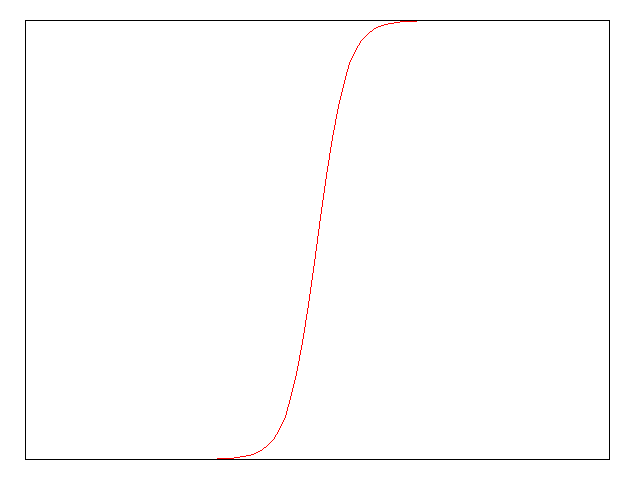
\includegraphics[width=0.5\textwidth]{kink.png}
    \caption{Kink Solution}
    \label{fig:q2_kink}
\end{figure}

\begin{figure}[H]
    \centering
    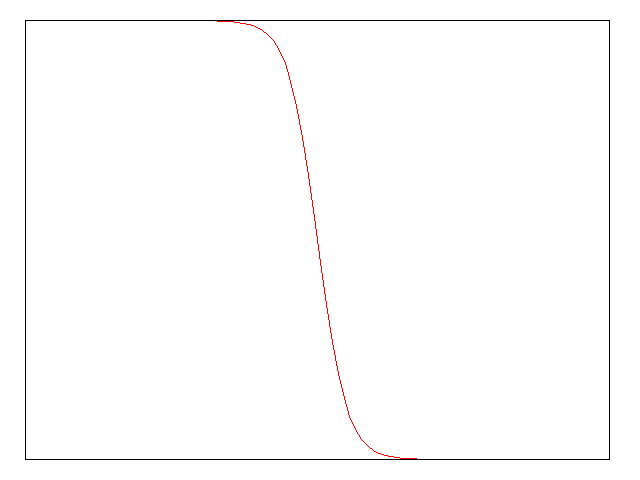
\includegraphics[width=0.5\textwidth]{anti_kink.png}
    \caption{Anti-Kink Solution}
    \label{fig:q2_anti_kink}
\end{figure}

\begin{figure}[H]
    \centering
    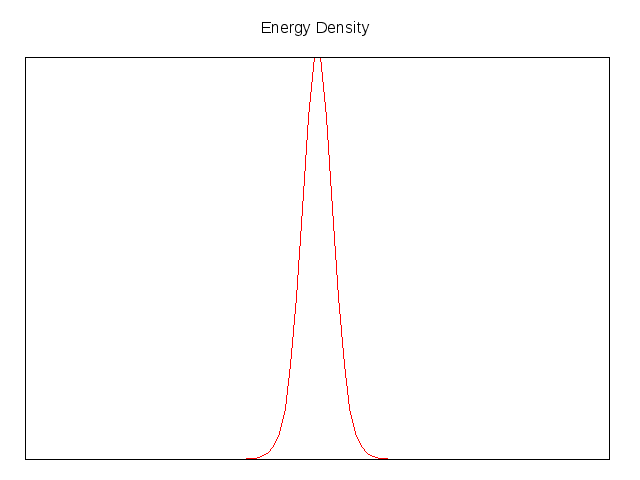
\includegraphics[width=0.5\textwidth]{energy_density.png}
    \caption{Energy Density}
    \label{fig:q2_anti_kink}
\end{figure}
